% ########################################################################################################################################
%
% This is the main latex file. Here we call for inputs from other files. We also define some of the main characteristics of the document.
%
% ########################################################################################################################################
%
% You likely only need to modify the "Main_Content__Write_your_essay_here.tex" file.
%
% ########################################################################################################################################

\documentclass[12pt,a4paper,oneside]{paper}
%TC:ignore
% ################################################################################
% 
%       INSTRUCTIONS, PLEASE READ BEFORE IF YOU INTEND TO MODIFY THIS FILE
% 
% ################################################################################
% For the most part, you should not change this file. In particular, the format 
% should not be changed. However, depending on what you want you might need to
% use additional packages (and possibly remove old ones that may be incompatible.
% Do that at your own discretion.
% ################################################################################

% Encoding and Language
\usepackage[utf8x]{inputenc}
\usepackage{csquotes}
\usepackage[main=portuguese]{babel}
\usepackage{iflang}

% Font Configurations
\renewcommand{\rmdefault}{phv}
\renewcommand{\sfdefault}{phv}
\def\FontLn{% 16 pt normal
  \usefont{T1}{phv}{m}{n}\fontsize{14pt}{14pt}\selectfont}
\def\FontLb{% 16 pt bold
  \usefont{T1}{phv}{b}{n}\fontsize{14pt}{14pt}\selectfont}
\def\FontMn{% 14 pt normal
  \usefont{T1}{phv}{m}{n}\fontsize{12pt}{12pt}\selectfont}
\def\FontMb{% 14 pt bold
  \usefont{T1}{phv}{b}{n}\fontsize{12pt}{12pt}\selectfont}
\def\FontSn{% 12 pt normal
  \usefont{T1}{phv}{m}{n}\fontsize{10pt}{10pt}\selectfont}

% Font Encoding
\usepackage[T1]{fontenc}

% Page Geometry
\usepackage{geometry}	
\geometry{verbose,tmargin=2cm,bmargin=1.7cm,lmargin=2cm,rmargin=2cm}
\usepackage{multirow}
\usepackage{multicol}

% Line Spacing
\usepackage{setspace}
\renewcommand{\baselinestretch}{1.2}

% Graphics and Figures
\usepackage{graphicx}
\usepackage{subfigure}
\usepackage{subfigmat}
\usepackage{float}

%Colors
\usepackage{xcolor}

% Mathematics and Theorems
\usepackage{amsmath}
\usepackage{amsthm}
\usepackage{amsfonts}
\usepackage{dcolumn}
\usepackage{indentfirst}

% Comments and Verbatim
\usepackage{verbatim}

% Hyperlinks
\usepackage[pdftex]{hyperref}
\hypersetup{
    colorlinks,
    linkcolor=blue,
    anchorcolor=black,
    citecolor=cyan,
    filecolor=black,
    menucolor=black,
    urlcolor=teal,
    bookmarksopen=true,
    bookmarksnumbered=true
}

% Captions and References
\usepackage[figure,table]{hypcap}
\usepackage[format=plain]{caption}
\DeclareCaptionFont{georgia}{\small\fontseries{n}\fontfamily{georgia}\selectfont}
\captionsetup{labelfont=georgia,font=georgia}

% Bibliography
\usepackage[backend=biber,style=apa]{biblatex}

% Index
\usepackage{makeidx}
\makeindex

% Acronyms
\usepackage[printonlyused]{acronym}

% Lipsum (for placeholder text)
\usepackage{lipsum}

% Cleveref (for clever references)
\usepackage[\IfLanguageName{english}{english}{portuguese}]{cleveref}

% Colors
\usepackage{xcolor}
\usepackage{color}

% Custom Commands
\newcommand{\gray}[1]{\textcolor{gray}{#1}}

% Equation Numbering
\renewcommand{\theequation}{{\fontseries{n}\fontfamily{georgia}\selectfont\arabic{equation}}}

% Section and Subsection Fonts
\sectionfont{\Large\bfseries\fontfamily{lmss}\selectfont}
\subsectionfont{\large\bfseries\fontfamily{lmss}\selectfont}
%TC:endignore


\addbibresource{bibliography.bib}
\begin{document}
\pagestyle{fancy}
\fancyhf{} % Clear previous settings
\rhead{LIFE}
\lhead{Millikan}

%TC:ignore
% #############################################################################
%
%                           ENTER YOUR NAME, ISTid, AND TITLE
% 
% #############################################################################



\def\title {}


% #############################################################################
%
%               DO NOT MODIFY THE LINES FROM HERE TO THE MAIN DOCUMENT BODY
% 
% #############################################################################

\thispagestyle {empty}
\begin{center}
\begin{minipage}[c][5cm][t]{\textwidth}
\begin{center}

\includegraphics[width=5cm]{../IST_A_RGB_POS.png}
\end{center}

\end{minipage}
\begin{minipage}[t][10cm][c]{\textwidth}
\centering
{\FontMb Instituto Superior Técnico} \\
\paragraph{}
\centering
{\FontLb\Huge \title{}}
\paragraph{}
\centering
{\FontMb Laboratório de Introdução à Física Experimental} \\
\paragraph{}
{\FontMb 2023/2024}
\end{minipage}

\begin{minipage}[c][2cm][c]{\textwidth}
\centering
{\FontLn }
\end{minipage}
\begin{minipage}[c][2cm][c]{\textwidth}
\centering
\end{minipage}
\begin{minipage}[c][1cm][c]{\textwidth}
\centering
\fbox{{\FontMb Report}}
\end{minipage}
\begin{minipage}[c][3cm][c]{\textwidth}
\centering
{\FontMb
102716 Pedro Curvo}
\end{minipage}
\begin{minipage}[c][2cm][c]{\textwidth}
\centering

\end{minipage}

\end{center} 
\normalsize
\cleardoublepage
\setcounter{page}{1}
\fontfamily{cmr}\selectfont
%TC:endignore
% #############################################################################
%
%                           BEGIN MAIN DOCUMENT BODY
%
% #############################################################################

\printindex


\section{\sf Conceitos fundamentais}
%\section{\sf }
%\subsection{\sf }
\subsection{\sf Corpo esférico em queda livre num fluido}
Um corpo de dimensões muito pequenas,\footnote{Com número de Reynolds $Re= \frac{\rho v L}{\eta}$ inferior a $\simeq 100$} 
ao mover-se com uma velocidade relativamente baixa através de um fluido (líquido ou gás), fica sujeito a uma força de atrito
aproximadamente proporcional à sua velocidade, modelada pela expressão:

\begin{equation}
	\label{eq:f_atrito}
	\vec{F}_{at} = - k \, \eta \vec{v}
\end{equation}
em que $\eta$ é o coeficiente de viscosidade do fluido, $\vec{v}$ é a velocidade do corpo e $k$ é um coeficiente que depende
da forma do corpo, que no caso deste ser uma esfera de raio $R$ toma o valor (lei de Stokes): 
\begin{equation}
	\label{eq:coef_atrito}
	k = 6 \pi R
\end{equation}


O coeficiente $k$ virá assim expresso em \emph{metro} no Sistema Internacional (SI) e o coeficiente de viscosidade em Pa$\cdot$s
(ou N$\cdot$s/m$^2$).
Normalmente a unidade de viscosidade que aparece na literatura é a unidade do sistema C.G.S. (g/cm$\cdot$s) que é designada por
Poise (abreviatura P), verificando-se então a equivalência:

\begin{equation*}
	1 \, \mathrm{P} = 0,1\, \mathrm{Pa}\cdot\mathrm{s}
\end{equation*}

Quando um corpo de massa $m$ cai em queda livre sob a ação do seu peso ($\vec{P}=m\vec{g}$) através de um fluido, o seu
movimento de queda será abrandado pela força de atrito, e a equação do movimento escreve-se:

\begin{equation}
	\label{eq:mov}
	m\,a \equiv m\, \frac{dv}{dt} =  m\,g - k  \, \eta \, v
\end{equation}

A partir de uma velocidade inicial nula, e sendo o peso do corpo constante, a aceleração $a$ produz um aumento  em $v(t)$
e, por consequência, um aumento na força de atrito $F_{at}$. Para uma determinada velocidade limite $v_L$, o segundo membro
de (\ref{eq:mov}) anula-se e o corpo passará a deslocar-se com movimento uniforme. A velocidade limite $v_L$ será então obtida
fazendo $a= 0$ na equação (\ref{eq:mov}):

\begin{equation}
	\label{eq:vlimit}
	v_L = \frac{m\,g}{k  \, \eta}
\end{equation}
o que poderá ser facilmente constatado pela resolução\footnote{Ver notas de apoio às aulas teóricas} da equação (\ref{eq:mov}),
cuja solução é da forma:

\begin{equation}
	\label{eq:vlimita}
	v(t) = \frac{m\,g}{k  \, \eta} (1 - e^{- (k\,\eta / m) t}) = v_L (1-e^{-t/\tau})
\end{equation}
à qual corresponde o gráfico  da Fig~\ref{fig:vLim}, e onde se definiu o tempo caraterístico $\tau=k\eta/m$. Quando
$t \to \infty$ temos $v(t) \to v_L = \frac{m\,g}{k  \, \eta} $.


%\end{multicols}

\begin{figure}[H]
  \centering 
	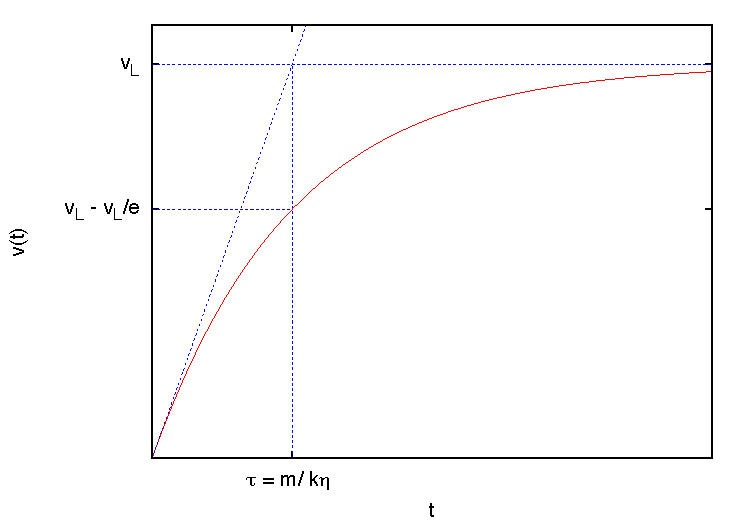
\includegraphics[width=0.6\textwidth]{./milikan_images/plote}
	\caption{ Evolução da velocidade de um corpo em queda livre sujeito a uma força de atrito. \label{fig:vLim}} 
\end{figure}

%\begin{multicols}{2}

Se pretendermos ser mais rigorosos, devemos substituir  em (\ref{eq:vlimit}) o peso do corpo pelo seu “peso aparente” no
fluido. De fato, um corpo em queda livre através de um fluido experimenta, além da ação da força de atrito, outra força de
baixo para cima cujo módulo é igual ao peso do fluido deslocado pelo corpo, de acordo com o Princípio de Arquimedes. Assim,
as equações (\ref{eq:mov}) e (\ref{eq:vlimit}) deverão ser modificadas para:

\begin{equation}
	\label{eq:mov2}
	m\,a = m\,g - m_f\,g  - k  \, \eta \, v
\end{equation}
\begin{equation}
	\label{eq:vlimit2}
	v_L = \frac{(m - m_f)\,g}{k  \, \eta}
\end{equation}
onde $m_f$ é a massa do fluido deslocado. No caso de um corpo esférico de raio $R$, introduzindo a equação (\ref{eq:coef_atrito})
em (\ref{eq:vlimit2}) e atendendo a que:

\begin{equation*}
	m = \frac{4}{3} \pi R^3 \rho \quad \textrm{  e } \quad  m_f = \frac{4}{3} \pi R^3 \rho_f
\end{equation*}
obtemos
\begin{equation}
	\label{eq:vlimit3}
	v_L = \frac{2\,R^2\, (\rho - \rho_f)\,g}{9  \, \eta}
\end{equation}
em que $\rho$  e $\rho_f$ são as massas específicas do corpo e do fluido. Note-se que conhecendo o raio do corpo é pois possível
determinar  a sua velocidade limite de queda, e vice-versa.

%

%\end{multicols}

\begin{figure}[H]
	[tb]  \centering 
	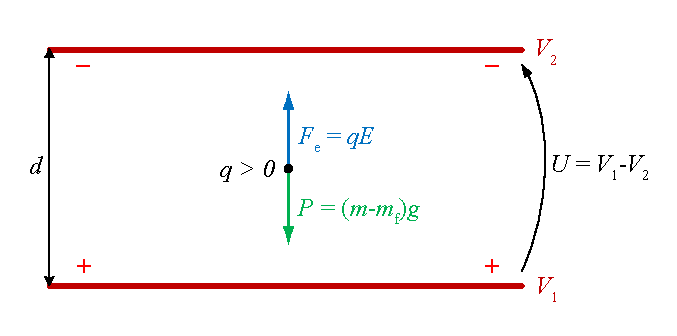
\includegraphics[width=0.7\textwidth]{./milikan_images/F_equil}
	\caption{Equilíbrio de forças numa gota sujeita a campos gravítico e elétrico. \label{fig:f_equil}} 
\end{figure}

%\begin{multicols}{2}

\subsection{\sf Equilíbrio dum corpo carregado, imerso num fluido, através de um campo elétrico vertical}

Considere o esquema representado na figura \ref{fig:f_equil}, em que um fluido não condutor se encontra entre duas placas
condutoras paralelas separadas de uma distância $d$. Ao aplicar-se uma diferença de potencial \mbox{$U = V_1 -V_2 > 0$} com a
polaridade indicada na figura, é criado um campo elétrico ascendente. Se entre as placas se encontrar uma partícula de massa $m$
e carga positiva\footnote{No caso da partícula estar carregada negativamente obteríamos o mesmo resultado invertendo o sentido do
campo elétrico.} $q$  esta ficará sujeita a uma força elétrica que contrariará a sua queda.
Na hipótese do campo elétrico ser uniforme\footnote{Nomeadamente, se a distância entre as placas for muito menor que as suas
dimensões laterais.} o módulo de $\vec{E}$ e o módulo da força elétrica $\vec{F}_e$ que atua na partícula serão dados por:
\begin{equation*}
	E = \frac{U}{d}, \qquad  F_e = |q| \frac{U}{d}
\end{equation*}

Assim, a queda da partícula será agora contrariada pela força elétrica e pela força de atrito.
A equação (\ref{eq:mov2}) passa a escrever-se:

\begin{equation}
	\label{eq:mov3}
	m\,a = (m - m_f)\,g  - q \frac{U}{d} - k  \, \eta_{ar} \, v
\end{equation}
Variando a diferença de potencial (ddp) $U$, pode-se estabelecer o equilíbrio entre o peso da partícula e a força elétrica,
conseguindo-se a sua paragem entre as placas. Nessa situação, tem-se simultaneamente $F_{at}=0$, $a=0$ e  $v$  $=0$:

\begin{equation}
	\label{eq:equil}
	0 = (m - m_f)\,g  - q \frac{U}{d} 
\end{equation}
Nesta equação a expressão $(m - m_f)\,g$ pode ser substituída usando a equação (\ref{eq:vlimit2}), obtendo-se:

\begin{equation*}
	v_L\, k\, \eta_{ar} = q \frac{U}{d}
\end{equation*}
E entrando também com a eq. (\ref{eq:coef_atrito}) no caso de a partícula ser esférica, obtemos por fim:

\begin{equation}
	\label{eq:carga}
	q = \frac{6 \pi \, R \, \eta_{ar} \, d\, v_L}{U}  
\end{equation}
onde

\begin{itemize}
\item $v_L$, a velocidade limite de queda da partícula através do fluido, na ausência do campo elétrico
\item $\eta_{ar} = 18,52 \cdot 10^{-5}$ P$ =  18,52 \cdot 10^{-6} \;$ Pa$\cdot$s (viscosidade do ar a 23 $^{\circ}$C)
\item $\rho = 973 \,$ kg/m$^{3}$ (massa específica do óleo de silicone)
\item $\rho_f = 1 \,$ kg/m$^{3}$ (massa específica do ar)
\item $g=9,80\,$ m/s$^{2}$ (aceleração gravítica em Lisboa)
\item $d$ (distância entre placas, a medir no laboratório)
\end{itemize}

\subsection{\sf Correções}
\subsubsection{\sf Temperatura ambiente}

No caso da temperatura ambiente se afastar muito de $23\,^{\circ}\mathrm{C}$, o valor  da viscosidade do ar terá de ser
corrigido.\footnote{Utilize por exemplo a calculadora \emph{online}: http://www.lmnoeng.com/Flow/GasViscosity.htm}

\subsubsection{\sf Dimensão das gotas}

A Lei de Stokes não é exata quando as dimensões dos corpos esféricos forem comparáveis à distância média entre as moléculas
do ar. Nestas condições, Millikan verificou que a viscosidade $\eta_{ar}$ deveria ser substituída por:

\begin{equation}
	\label{eq:correcao}
	\eta_{ar}' = \frac{\eta_{ar}}{1 + b/(p\,R)}  
\end{equation}
em que a constante $b=7,88\cdot 10^{-3}$ Pa$\cdot$m, 
$p$ é pressão atmosférica expressa em pascal e $R$ é o raio da gota em metros.
%$0.000617$, $p$ é pressão expressa em $cm$ de %mercúrio\footnote{$1\,atm  = 1.013 \times 10^5 \,Pa = %1013 \, mbar %= 76\, cm_{Hg}$}  e $R$ é o raio da gota em %$cm$.

O valor corrigido $q'$ será  determinado a partir do valor experimental $q$ por

\begin{equation}
	\label{eq:correcao1}
	q' = q\, \left(\frac{\eta_{ar}'}{\eta_{ar}}\right)^{3/2}  =q\, \left(\frac{1}{1 + b/(p\,R)}\right)^{3/2}  
\end{equation}

\section{\sf Figuras dos aparelhos da montagem experimental}
\begin{figure}[H]
	[htb]  \centering 
	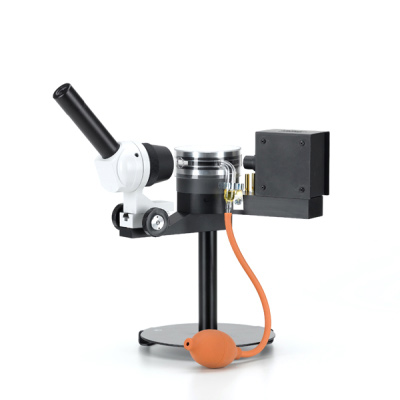
\includegraphics[width=0.5\textwidth]{./milikan_images/U131001_01_Aparelho-de-Millikan.jpg}
	\caption{Equipamento para determinação da carga das gotas. \label{fig:Equi}} 
\end{figure}

\begin{figure}[H]
	[htb]  \centering 
	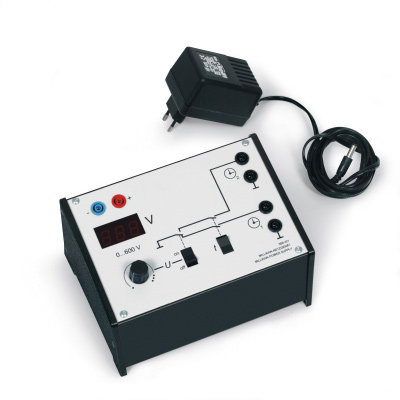
\includegraphics[width=0.5\textwidth]{./milikan_images/U13105-230_01_Aparelho-operacional-de-Millikan.jpg}
	\caption{Gerador de alta tensão DC regulável. \label{fig:fonteDC_HT}} 
\end{figure}


\newpage
\section{\sf Procedimento experimental}


\subsection{\sf Material}

\begin{enumerate}
	\item Célula de Millikan com gerador de alta tensão DC regulável
	\item  Atomizador e óleo de silicone
	\item Cronómetro
	\item Nível de bolha de ar% Parafuso para calibração do retículo do microscópio
\end{enumerate}


\subsection{\sf Trabalho preparatório} 
\begin{enumerate}
\item Preencha os objetivos do trabalho que irá realizar na sessão de laboratório. 
\item Preencha o quadro com as equações necessárias para o cálculo das grandezas, bem como as suas incertezas. 
\end{enumerate}

\subsection{\sf Montagem experimental}
Efetue a montagem de acordo com a Fig. \ref{fig:esquema-millikan}. Chame o professor antes de ligar os aparelhos à corrente
elétrica.

\begin{figure}[H]
	[htb]  \centering 
	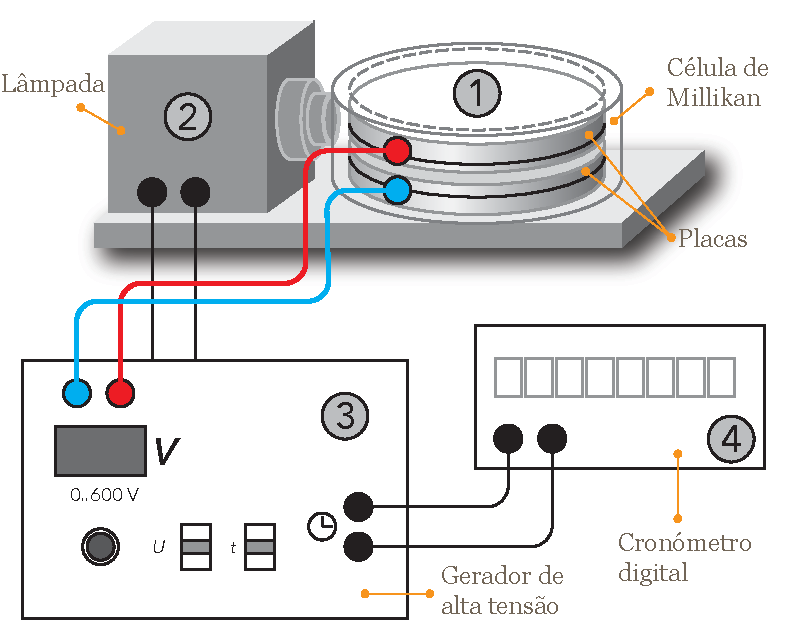
\includegraphics[width=0.6\textwidth]{./milikan_images/Esquema-Millikan.pdf}
	\caption{Esquema da montagem da experiência de Millikan. 1 - Célula de Millikan; 2 - lâmpada; 3 - gerador de alta tensão
    regulável; 4 - cronómetro.\label{fig:esquema-millikan}} 
\end{figure}



\subsection{\sf Determinação da tensão de equilíbrio}
\begin{enumerate}
\item   Depois de verificar que a célula está horizontal, meça o distância entre placas, $d$. Visualizando no computador,
tente focar o microscópio na zona onde as gotas irão ``flutuar''. Atenção: o microscópio amplia a imagem e a escala por 2$\times$.

\item Coloque o potenciómetro que controla a alimentação das placas do condensador no valor mínimo de tensão elétrica. 

\item    Verifique se o interruptor de inversão da alimentação do condensador está na posição ``Neutra''. Rode o potenciómetro
para uma posição que permita, quando ligar o interruptor de inversão, estabelecer um campo elétrico entre as placas do condensador. 

\item     Utilizando o pulverizador junto do orifício da célula, produza uma pequena ``nuvem'' de gotículas de óleo. Observe
através do microscópio o movimento das gotículas em frente do retículo, ajustando a focagem se necessário.

\item     Ligando o interruptor e variando a intensidade  e o  sentido do campo elétrico, verifique se existem gotículas eletrizadas. 

 \item Escolha uma das gotas e, ajustando a tensão, manipule a sua posição vertical de modo a que esta fique colocada numa
 determinada divisão do topo do retículo, imobilizando-a de seguida. Registe o valor da tensão. 
 \end{enumerate}
 
 \subsection{\sf Determinação da velocidade limite e da carga}
 \begin{enumerate}
 \setcounter{enumi}{6}

\item Anule o campo elétrico  e verifique que a gota cai sob acção da gravidade (com velocidade limite). 
Com um cronómetro ou gravando no computador e analisando o vídeo, meça o tempo necessário para que a gota percorra  $N>4$ divisões
do retículo. 
\item Repondo o campo elétrico, conduza a gota para a posição inicial para  medir o tempo pelo menos duas vezes. 

\item Repita este processo para várias gotas, tentando escolher as gotas de menor carga.

\item   Para cada gota, calcule a velocidade limite média e a respetiva incerteza, usando esse valor para estimar o raio e 
a carga. Calcule a carga corrigida pela viscosidade.

\item De modo a obter resultados mais fiáveis, tente assegurar-se de que as diversas gotas apresentam valores experimentais
diferentes. Duas gotas com valores da velocidade limite e raio muito semelhantes têm provavelmente a mesma carga, pelo que deverá repetir as medições para uma gota diferente.
\end{enumerate}

\subsection{\sf Análise, conclusões e comentários finais}
Discuta a qualidade dos dados obtidos e as conclusões que pode retirar desta experiência. Comente também sobre as condições
de realização da experiência, dos equipamentos utilizados e a influência de erros aleatórios e sistemáticos, identificando-os. Supondo que não conhecia o valor tabelado da carga do eletrão, e apenas a partir dos resultados obtidos, poderá tirar conclusões sobre a quantificação da carga elétrica?

\end{document}